\documentclass[12pt,]{article}
\usepackage[utf8]{inputenc}
\usepackage[T1]{fontenc}
\usepackage{mathptmx}
\usepackage{geometry}
\usepackage{mathtools}
\usepackage[english]{babel}
\usepackage{graphicx}
\usepackage[os=win]{menukeys}
\usepackage[figurename=Gambar]{caption}
\usepackage{hyperref}
\usepackage{minted}
\usepackage{float}
\usepackage{pdflscape}
\usepackage{pdfpages}
\usepackage{tikz}

\addto\captionsenglish{\renewcommand{\contentsname}{Daftar Isi}}
\addto\captionsenglish{\renewcommand{\bibname}{Referensi}}

\hypersetup{
	colorlinks=true, %set true if you want colored links
	linktoc=all,     %set to all if you want both sections and subsections linked
	linkcolor=blue,  %choose some color if you want links to stand out
}

\geometry{
	a4paper,
	left=15mm,
	right=10mm,
	top=10mm,
	bottom=10mm,
}

\usetikzlibrary{positioning}
\tikzstyle{squared} = [rectangle, rounded corners, minimum width=1cm, minimum height=0.5cm,text centered, draw=black]
\tikzstyle{connect} = [ultra thick,->]
\tikzstyle{connect2} = [ultra thick,<->]

\title{\Large \bf
	Pengenalan Pemrograman C dan chip seri ATMega.
}

\author{Achmadi ST MT}
\date{}

\begin{document}
	\maketitle
	\thispagestyle{empty}
	\pagestyle{empty}
	
	\newpage
	\tableofcontents
	
	\newpage
	\section{Requirement}
	
	Dalam pengembangan aplikasi berbasis ATMega, dibutuhkan beberapa hardware dan software.
	Berikut akan disebutkan dan dijelaskan untuk beberapa sistem operasi:
	
	\subsection{Software}
	
	\subsubsection{Code::Blocks}
	Code::Blocks adalah suatu program lingkungan pengembangan terpadu bebas, gratis, bersumber terbuka dan lintas platform.
	Program yang ditulis dalam C++ beserta wxWidgets untuk GUI-nya ini bisa digunakan bersama dengan berbagai macam kompilator, contohnya GCC dan CLang.
	Peralatannya yang tersedia tergantung dari "plugin" yang ada dipasang.
	Sekarang ini, Code::Blocks lebih tersedia sebagai perangkat pengembangan dalam bahasa C dan C++, walaupun program ini juga bisa disesuaikan, 
	dan mungkin akan membutuhkan pemasangan tambahan, untuk pengembangan perangkat lunak ARM, AVR, Fortran, GLFW, GLUT, GTK+,  MATLAB, OGRE, OpenGL, Qt, atau SDL.
	Code::Blocks tersedia di sistem operasi Windows, Linux, Mac OS X dan FreeBSD.
	\begin{figure}[H]
		\centering
		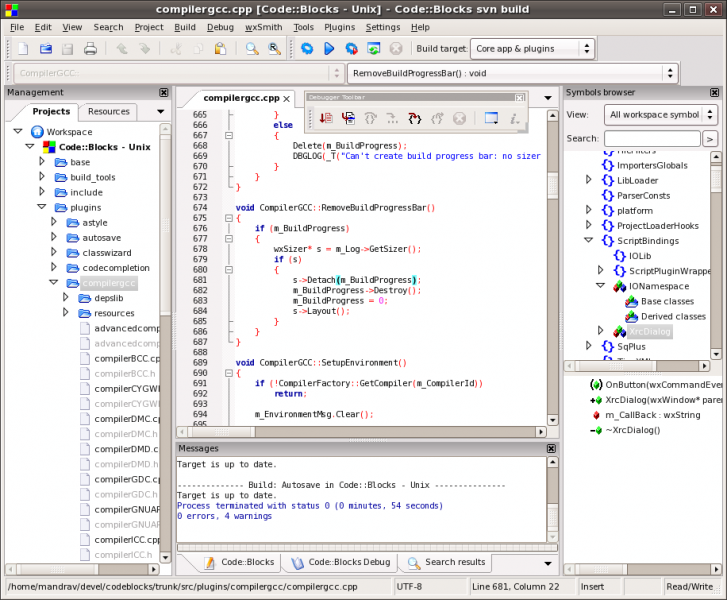
\includegraphics[width=0.6\linewidth]{images/cb}
		\caption{contoh tampilan Code::Blocks}
	\end{figure}

	Berikut instalasi:
	\begin{itemize}
		\item Windows.
		\begin{itemize}
			\item Buka alamat \url{http://www.codeblocks.org/downloads/26}.
			\item Klik file codeblocks-17.12mingw-setup.exe.
			\item Tunggu proses download selesai.
			\item Jalankan file codeblocks-17.12mingw-setup.exe untuk instalasi.
		\end{itemize}
	
		\item Ubuntu/Debian.
		\begin{itemize}
			\item Buka Terminal (pastikan terhubung internet).
			\item Masukkan perintah.
				\begin{minted}[frame=lines,fontsize=\footnotesize]{bash}
sudo apt-get install codeblocks build-essential
				\end{minted}
			\item Tunggu proses selesai.
		\end{itemize}
	
		\item Fedora.
		\begin{itemize}
			\item Buka Terminal (pastikan terhubung internet).
			\item Masukkan perintah.
				\begin{minted}[frame=lines,fontsize=\footnotesize]{bash}
sudo dnf groupinstall 'Development Tools'
sudo dnf install codeblocks
				\end{minted}
			\item Tunggu proses selesai.
		\end{itemize}
	
		\item Arch-Linux.
		\begin{itemize}
			\item Buka Terminal (pastikan terhubung internet).
			\item Masukkan perintah.
			\begin{minted}[frame=lines,fontsize=\footnotesize]{bash}
sudo pacman -S codeblocks base-devel 
			\end{minted}
			\item Tunggu proses selesai.
		\end{itemize}

	\end{itemize}

	\subsubsection{GCC AVR}
	GCC adalah software kompilasi gratis dan bebas untuk chip AVR.
	GCC (GNU C Compiler) bertugas mengkompilasi kode sumber menjadi file \textit{binary} yang siap dijalankan atau di-\textit{download} ke dalam chip.

	Berikut instalasi:
	\begin{itemize}
		\item Windows.
		\begin{itemize}
			\item Download file instalasi di alamat:
			\begin{itemize}
				\item Windows x86 (32bit): \url{http://blog.zakkemble.net/download/avr-gcc-8.3.0-x86-mingw.zip}
				\item Windows x64 (64bit): \url{http://blog.zakkemble.net/download/avr-gcc-8.3.0-x64-mingw.zip}
			\end{itemize}
			\item Extrak file yang sudah di download.
			\item Masukkan alamat kompiler dalam \textit{binary path} milik Windows.
		\end{itemize}
	
		\item Ubuntu/Debian.
		\begin{itemize}
			\item Buka Terminal (pastikan terhubung internet).
			\item Masukkan perintah.
			\begin{minted}[frame=lines,fontsize=\footnotesize]{bash}
sudo apt-get install gcc-avr binutils-avr avr-libc
			\end{minted}
			\item Tunggu proses selesai.
		\end{itemize}
		
		\item Fedora.
		\begin{itemize}
			\item Buka Terminal (pastikan terhubung internet).
			\item Masukkan perintah.
			\begin{minted}[frame=lines,fontsize=\footnotesize]{bash}
sudo dnf install avr-binutils avr-gcc avr-libc
			\end{minted}
			\item Tunggu proses selesai.
		\end{itemize}
		
		\item Arch-Linux.
		\begin{itemize}
			\item Buka Terminal (pastikan terhubung internet).
			\item Masukkan perintah.
			\begin{minted}[frame=lines,fontsize=\footnotesize]{bash}
sudo pacman -S avr-binutils avr-gcc avr-lib 
			\end{minted}
			\item Tunggu proses selesai.
		\end{itemize}
			
	\end{itemize}

	\subsubsection{Downloader}
	Download adalah software bantu untuk download (memasukkan) binary hasil kompilasi ke dalam chip.
	Tersedia banyak software tergantung tipe hardware downloader yang dipakai.
	Untuk kursus ini, digunakan downloader berbasis UASAsp, maka software downloader yang digunakan adalah
	Khazama untuk Windows dan avrdude (AVR Downloader/UploaDEr) untuk selain Windows.
	
	Berikut instalasi:
	\begin{itemize}
		\item Windows
		\begin{figure}[H]
			\centering
			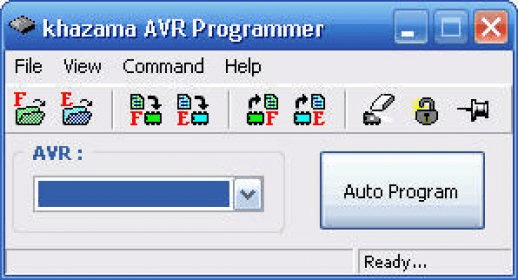
\includegraphics[width=0.4\linewidth]{images/khazama}
			\caption{contoh tampilan Khazama}
		\end{figure}
		\begin{itemize}
			\item Download file instalasi Khazama 1.6 di alamat \url{http://khazama.com/project/programmer/KhazamaAVRProgrammer162.rar}.
			\item Ekstrak file yang di download dan jalankan file installernya.
		\end{itemize}
	
		\item Ubuntu/Debian.
		\begin{itemize}
			\item Buka Terminal (pastikan terhubung internet).
			\item Masukkan perintah.
			\begin{minted}[frame=lines,fontsize=\footnotesize]{bash}
sudo apt-get install avrdude
			\end{minted}
			\item Tunggu proses selesai.
		\end{itemize}
		
		\item Fedora.
		\begin{itemize}
			\item Buka Terminal (pastikan terhubung internet).
			\item Masukkan perintah.
			\begin{minted}[frame=lines,fontsize=\footnotesize]{bash}
sudo dnf install avrdude
			\end{minted}
			\item Tunggu proses selesai.
		\end{itemize}
		
		\item Arch-Linux.
		\begin{itemize}
			\item Buka Terminal (pastikan terhubung internet).
			\item Masukkan perintah.
			\begin{minted}[frame=lines,fontsize=\footnotesize]{bash}
sudo pacman -S avrdude
			\end{minted}
			\item Tunggu proses selesai.
		\end{itemize}

	\end{itemize}

	\subsubsection{Simul-IDE}
	
	Dalam kursus ini, untuk awal pelatihan, digunakan Simulator untuk menjalankan dan menguji program AVR yang dibuat.
	Simulator yang dipilih disini adalah Simul-IDE. 
	Simul-IDE adalah simulator rangkaian elektronik Digital/Analog sederhana yang dapat berjalan secara \textit{real-time}.
	Simul-IDE dapat mendukung microcontroller seperti chip seri AVR ataupun PIC.
	
	\begin{figure}[H]
		\centering
		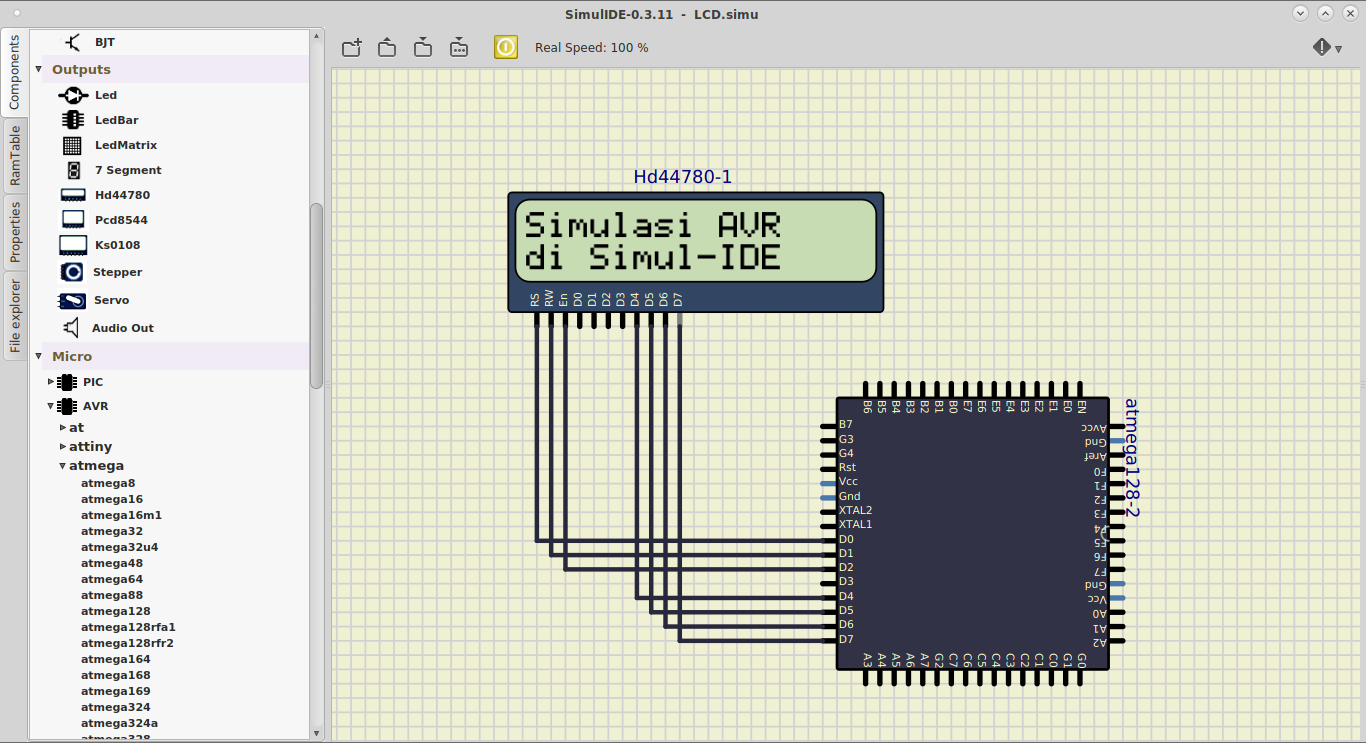
\includegraphics[width=0.6\linewidth]{images/simul}
		\caption{contoh tampilan Simul-IDE}
	\end{figure}

	Berikut untuk instalasi:
	\begin{itemize}
		\item Windows
		\begin{itemize}
			\item Buka alamat \url{https://sourceforge.net/projects/simulide/files/SimulIDE_0.3.10/SimulIDE_0.3.10_SR1-Win32.zip/download}
			\item Ekstrak file yang sudah di download.
			\item Jalankan file \textbf{run\_simulide.bat}.
		\end{itemize}
	
		\item Ubuntu/Debian.
		\begin{itemize}
			\item Buka Terminal (pastikan terhubung internet).
			\item Masukkan perintah.
			\begin{minted}[frame=lines,fontsize=\footnotesize]{bash}
sudo apt-get install simulide simavr
			\end{minted}
			\item Tunggu proses selesai.
			\item Buka terminal dimana project AVR berada.
			\item Masukkan perintah:
			\begin{minted}[frame=lines,fontsize=\footnotesize]{bash}
simulide
			\end{minted}
		\end{itemize}
	
		\item Fedora.
		\begin{itemize}
			\item Buka Terminal (pastikan terhubung internet).
			\item Masukkan perintah.
			\begin{minted}[frame=lines,fontsize=\footnotesize]{bash}
sudo dnf install simulide simavr
			\end{minted}
			\item Tunggu proses selesai.
			\item Buka terminal dimana project AVR berada.
			\item Masukkan perintah:
			\begin{minted}[frame=lines,fontsize=\footnotesize]{bash}
simulide
			\end{minted}
		\end{itemize}
	
		\item Arch Linux.
		\begin{itemize}
			\item Buka Terminal (pastikan terhubung internet).
			\item Masukkan perintah.
			\begin{minted}[frame=lines,fontsize=\footnotesize]{bash}
sudo pacman -S simavr
			\end{minted}
			\item Tunggu proses selesai.
			\item Download resep AUR di \url{https://aur.archlinux.org/cgit/aur.git/snapshot/simulide.tar.gz}
			\item Ekstrak file tersebut dan buka terminal di alamat tersebut.
			\item Masukkan perintah:
			\begin{minted}[frame=lines,fontsize=\footnotesize]{bash}
makepkg -sir
			\end{minted}
			\item Tunggu proses instalasi selesai
			\item Buka terminal dimana project AVR berada.
			\item Masukkan perintah:
			\begin{minted}[frame=lines,fontsize=\footnotesize]{bash}
simulide
			\end{minted}
		\end{itemize}
		
	\end{itemize}

	\subsubsection{KiCad}
	KiCad adalah software bebas dan gratis untuk membantu merancang circuit elektronik.
	KiCad menyediakan fitur olah skematik, layout PCB, dan 3D visualisasi.
	
	\begin{figure}[H]
		\centering
		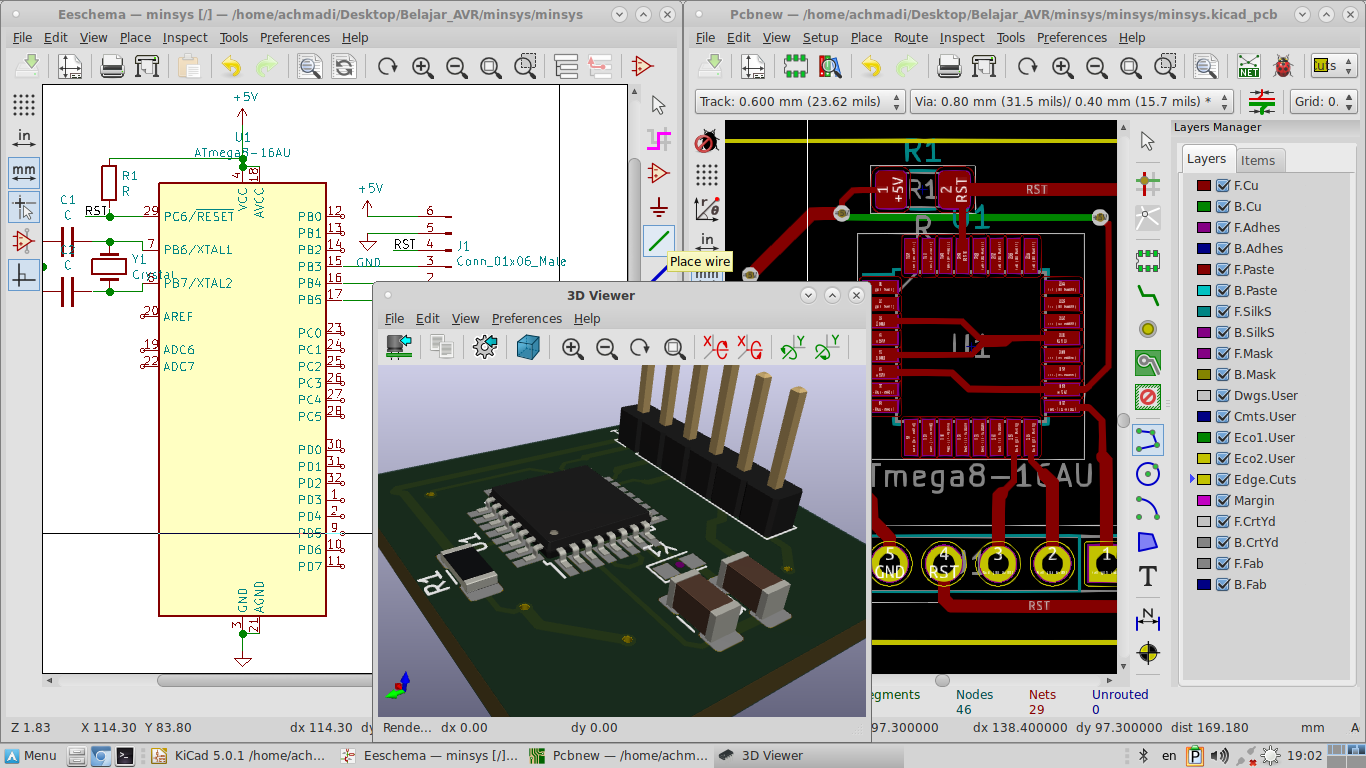
\includegraphics[width=0.6\linewidth]{images/kicad}
		\caption{contoh tampilan KiCAD}.
	\end{figure}

	Berikut untuk instalasi:
	\begin{itemize}
		\item Windows
		\begin{itemize}
			\item Buka alamat \url{http://kicad-pcb.org/download/windows/}
			\item Pilih dan download file instalasi sesuai laptop/komputer anda.
			\item Jalankan file instalasi.
		\end{itemize}
	
		\item Ubuntu/Debian.
		\begin{itemize}
			\item Buka Terminal (pastikan terhubung internet).
			\item Masukkan perintah.
			\begin{minted}[frame=lines,fontsize=\footnotesize]{bash}
sudo add-apt-repository ppa:js-reynaud/kicad-5
sudo apt-get update
sudo apt-get install kicad
			\end{minted}
			\item Tunggu proses selesai.
		\end{itemize}
		
		\item Fedora.
		\begin{itemize}
			\item Buka Terminal (pastikan terhubung internet).
			\item Masukkan perintah.
			\begin{minted}[frame=lines,fontsize=\footnotesize]{bash}
sudo dnf install kicad kicad-packages3d
			\end{minted}
			\item Tunggu proses selesai.
		\end{itemize}
		
		\item Arch Linux.
		\begin{itemize}
			\item Buka Terminal (pastikan terhubung internet).
			\item Masukkan perintah.
			\begin{minted}[frame=lines,fontsize=\footnotesize]{bash}
sudo pacman -S kicad kicad-library kicad-library-3d
			\end{minted}
			\item Tunggu proses selesai.
		\end{itemize}
		
	\end{itemize}

	\subsection{Hardware}
	
	Untuk hardware, kebutuhan pokok dalam membangun aplikasi ATMega hanyalah 2 saja, yaitu: Downloader dan Minimum-System 
	
	\subsubsection{Downloader}
	Downloader adalah hardware yang digunakan untuk memasukkan program dalam chip.
	Tipe downloader yang digunakan disini adalah USBAsp dimana baik skematik maupun firmware yang digunakan bersifat open-source.
	USBAsp secara mendasar hanya membutuhkan:
	\begin{itemize}
		\item ATMega48, ATMega8, atau ATMega88
		\item Clock 12MHz atau lebih
		\item 2 PIN untuk jalur VCC dan GND
		\item 4 PIN untuk jalur SPI (SS, MOSI, MISO, dan SCK)
		\item 4 PIN untuk jalur USB (VCC, GND, D+, dan D-)
	\end{itemize}
	Project USBAsp dapat anda temukan di alamat \url{https://www.fischl.de/usbasp/}.
	
	\begin{figure}[H]
		\centering
		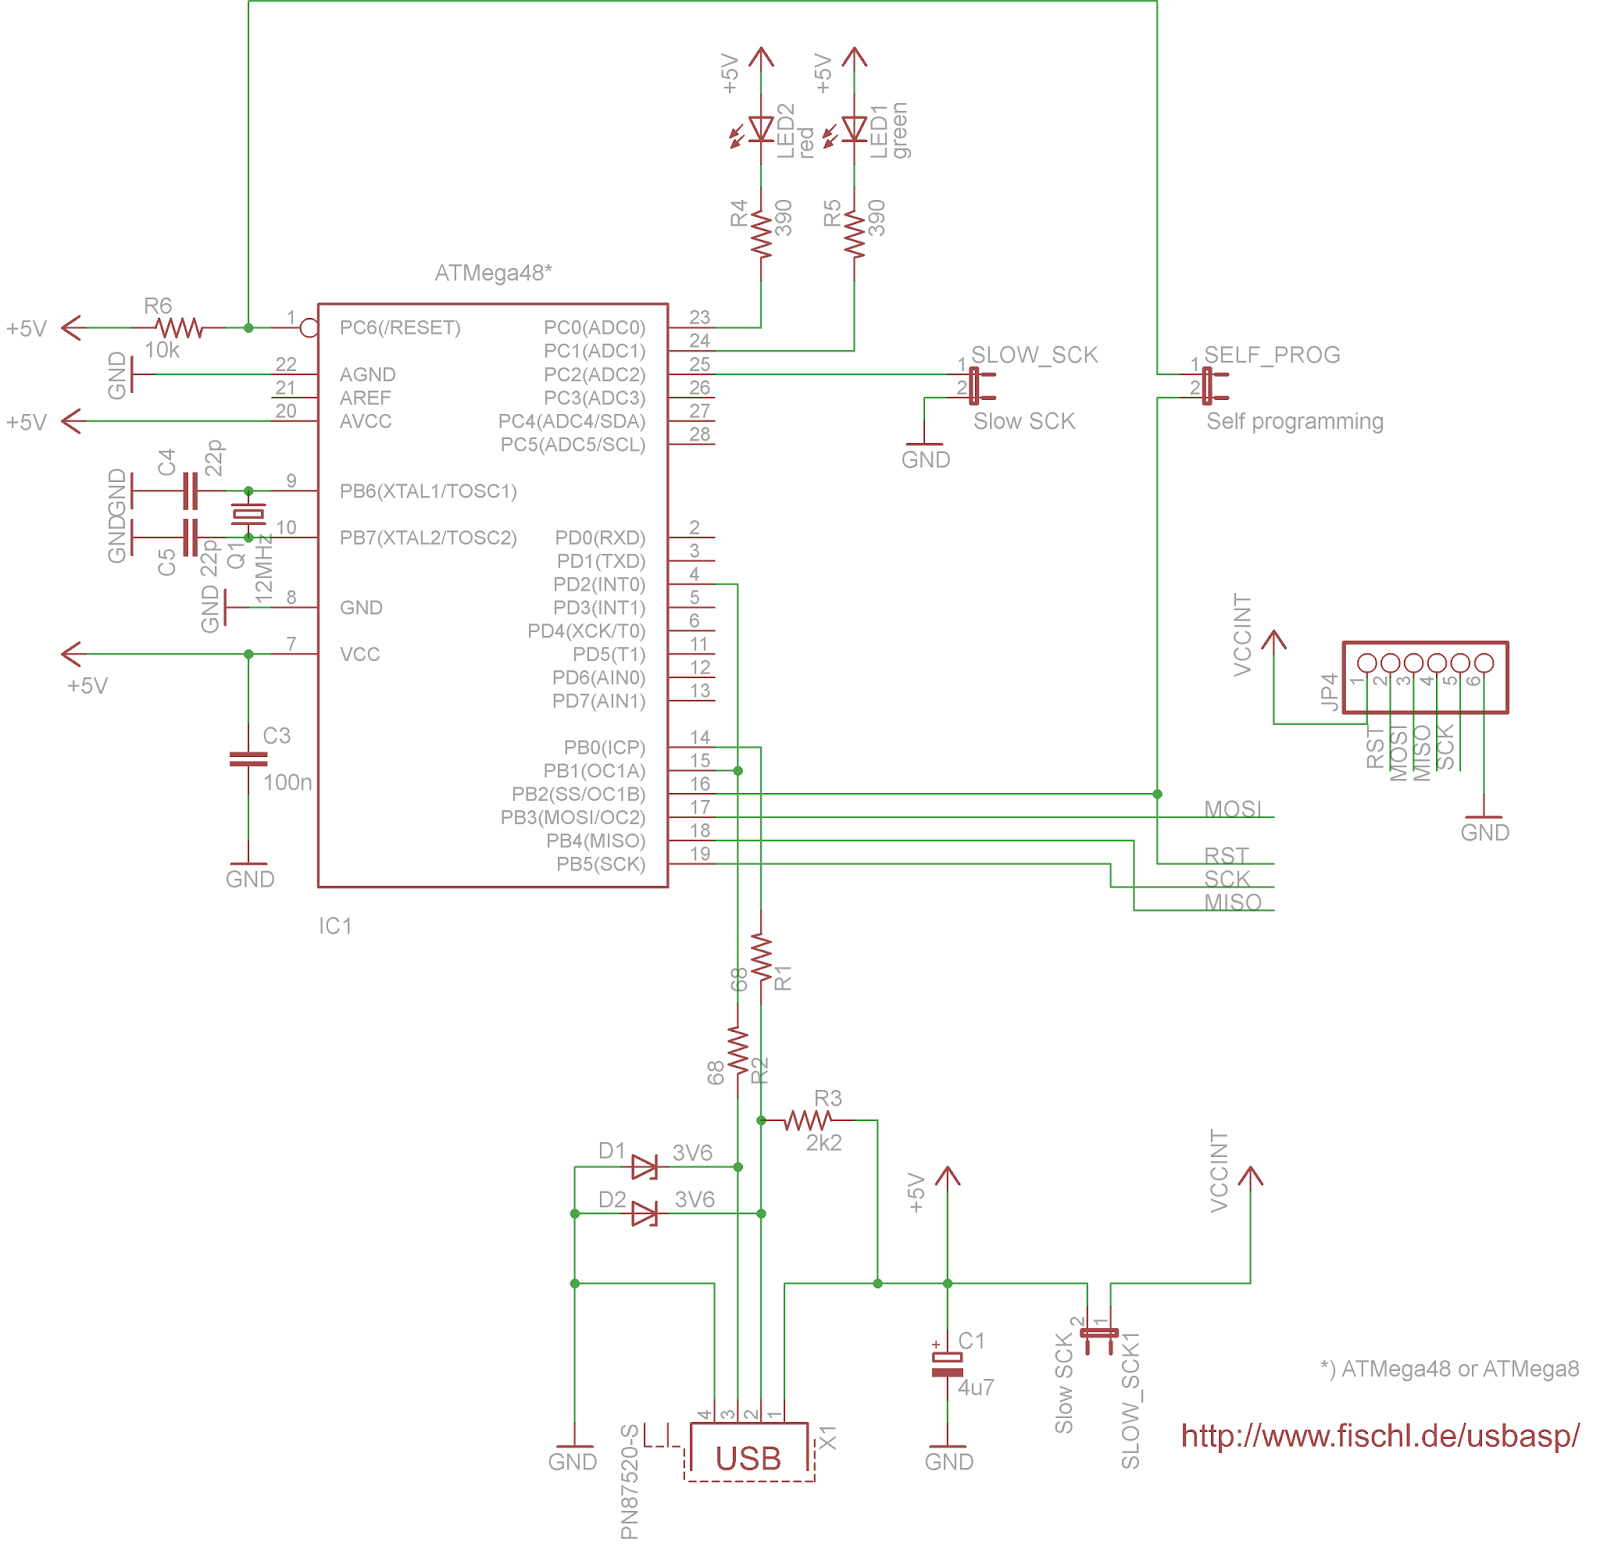
\includegraphics[width=0.6\linewidth]{images/usbasp}
		\caption{contoh skematik USBAsp}
	\end{figure}

	Sedangkan untuk hardware dapat anda beli di pasaran dengan harga terjangkau atau anda dapat merakit sendiri.
	
	\begin{figure}[H]
		\centering
		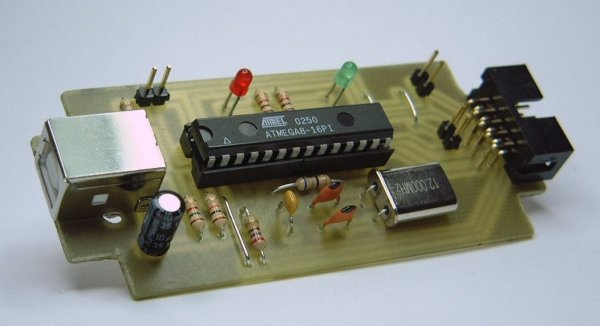
\includegraphics[width=0.6\linewidth]{images/usbasphard}
		\caption{contoh USBAsp murah meriah}
	\end{figure}

	\textbf{Advance}: Selain menggunakan USBAsp fisik, anda dapat juga menanamkan \textit{virtual} downloader USBAsp kedalam bagian \textit{bootloader} ATMega.
	Keuntungannya anda tidak lagi perlu USBAsp fisik terpisah dengan Minimum-System,
	namun kekurangannya adalah alamat aplikasi berpindah ke alamat bootloader sehingga terkadang memory tidak sampai alamat aplikasi.
	Project ini dikenal dengan USBAspLoader dan dapat anda temukan di \url{https://www.obdev.at/products/vusb/usbasploader.html}.
	
	\subsubsection{Minimum-System}
	Minimum-System didefiniskan sebagai rangkaian dasar agar chip ATMega dapat berjalan.
	Pada dasarnya ATMega hanya membutuhkan:
	\begin{itemize}
		\item Power VCC (5v) dan GND (0v). Power ini bisa didapat dari tegangan USB atau output regulator 7805/LM2569s.
		\item 5 PIN untuk download via SPI (GND, RST, MOSI, MISO, dan SCK) jika ingin didownload \textit{on-board}.
		\item Crystal (XTALL) atau RTC jika sumber Clock ATMega di set eksternal.
	\end{itemize}

	\begin{figure}[H]
		\centering
		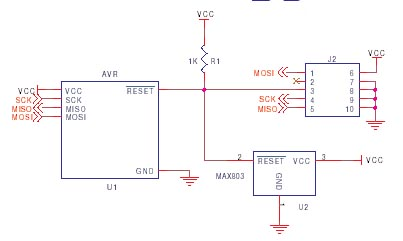
\includegraphics[width=0.6\linewidth]{images/minsys}
		\caption{contoh diagram dasar Minimum-System}
	\end{figure}

	Berdasarkan rangkaian dasar ini, anda dapat menambahkan beragam komponen lain sesuai kebutuhan anda.
	Jika anda tidak waktu untuk membangun Minimum-System sendiri, anda dapat membelinya di pasaran dengan beragam harga dan spesifikasi.
	
	\begin{figure}[H]
		\centering
		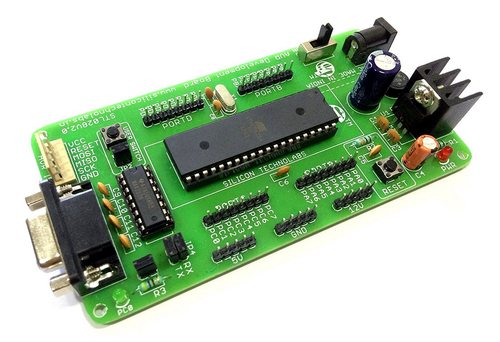
\includegraphics[width=0.6\linewidth]{images/minsyshard}
		\caption{contoh fisik Minimum-System yang dilengkapi RS-232 dan regulator 5v}
	\end{figure}

	\newpage
	\section{Bahasa C}
	Bahasa pemrograman C merupakan salah satu bahasa pemrograman komputer. Dibuat pada tahun 1972 oleh Dennis Ritchie untuk Sistem Operasi Unix di Bell Telephone Laboratories.
	
	Meskipun C dibuat untuk memprogram sistem dan jaringan komputer namun bahasa ini juga sering digunakan dalam mengembangkan software aplikasi.
	C juga banyak dipakai oleh berbagai jenis platform sistem operasi dan arsitektur komputer, bahkan terdapat beberepa compiler yang sangat populer telah tersedia.
	C secara luar biasa memengaruhi bahasa populer lainnya, terutama C++ yang merupakan extensi dari C.
	
	\subsubsection{Kompilasi}
	Kompilasi adalah proses mengumpulkan dan mengubah kode sumber menjadi file yang bisa dijalankan.
	Software/Firmware memiliki 2 bentuk yaitu kode sumber (\textit{source}) dan \textit{binary}.
	Source dapat dibaca oleh manusia, namun belum bisa dimengerti oleh CPU.
	Sebaliknya, binary tidak bisa dipahami manusia, namun bisa dipahami CPU dan dijalankan isinya. 
	Berikut secara ringkas diagram kompilasi:
	
	\begin{figure}[H]
		\begin{center}
			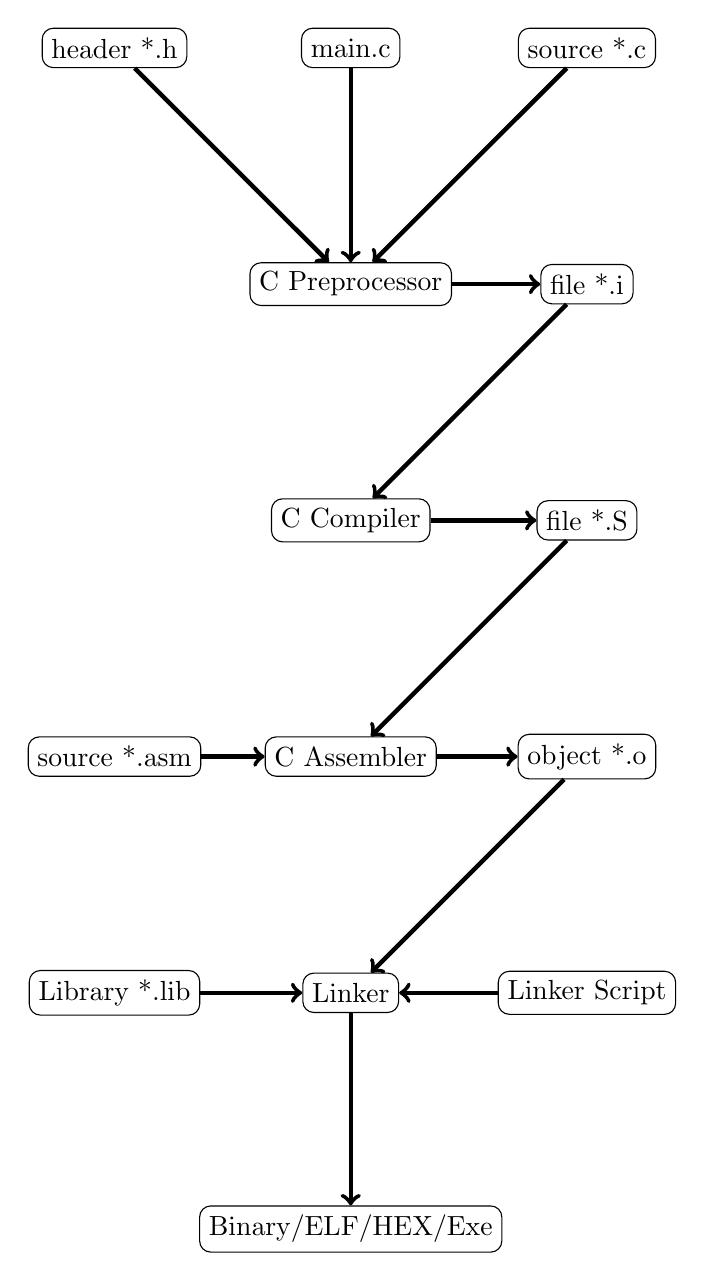
\begin{tikzpicture}[node distance=3cm]
			\node (mainc) [squared] {main.c};
			\node (cheader) [squared,left of=mainc] {header *.h};
			\node (csource) [squared,right of=mainc] {source *.c};
			\node (preproc)[squared,below of=mainc]{C Preprocessor};
			\node (cproc)[squared,right of=preproc]{file *.i};
			%-----------------------------------------------
			\node (cc) [squared,below of=preproc]{C Compiler};
			\node (casm) [squared,right of=cc]{file *.S};
			%-----------------------------------------------
			\node (asm) [squared,below of=cc]{C Assembler};
			\node (asmsource)[squared,left of=asm]{source *.asm};
			\node (obj)[squared,right of=asm]{object *.o};
			%-----------------------------------------------
			\node (linker) [squared,below of=asm]{Linker};
			\node (library) [squared,left of=linker]{Library *.lib};
			\node (linkscr) [squared,right of=linker]{Linker Script};
			%-----------------------------------------------
			\node (binary) [squared,below of=linker]{Binary/ELF/HEX/Exe};
			
			%-----------------------------------------------
			%-----------------------------------------------
			
			\draw [connect] (mainc) -- (preproc);
			\draw [connect] (cheader) -- (preproc);
			\draw [connect] (csource) -- (preproc);
			\draw [connect] (preproc) -- (cproc);
			\draw [connect] (cproc) -- (cc);
			\draw [connect] (cc) -- (casm);
			\draw [connect] (casm) -- (asm);
			\draw [connect] (asmsource) -- (asm);
			\draw [connect] (asm) -- (obj);
			\draw [connect] (obj) -- (linker);
			\draw [connect] (library) -- (linker);
			\draw [connect] (linkscr) -- (linker);
			\draw [connect] (linker) -- (binary);
			\end{tikzpicture}
			\caption{Diagram Proses Kompilasi}
		\end{center}
	\end{figure}

	\newpage
	\subsubsection{Struktur Dasar C}
	Bahasa C secara umum memiliki 4 bagian wajib, yaitu:
	\begin{itemize}
		\item Preprocessor
		\item Functions
		\item Variables
		\item Statement (Expressions atau Operation).
	\end{itemize}
	Setiap baris \textit{statement} diakhiri dengan tanda titik koma (;).
	
	Berikut adalah contoh dasar yang dapat dijalankan di Code::Blocks.
	\begin{enumerate}
		\item Buka Code::Blocks.
		\item Buat project baru.
		\begin{figure}[H]
			\centering
			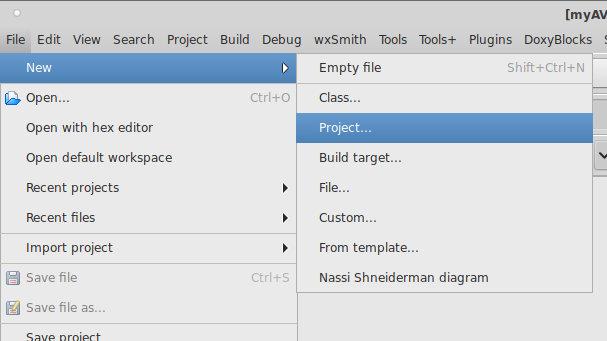
\includegraphics[width=0.5\linewidth]{images/c_cb_0}
			\caption{membuat project baru}
		\end{figure}
		\item Pilih Empty Project.
		\begin{figure}[H]
			\centering
			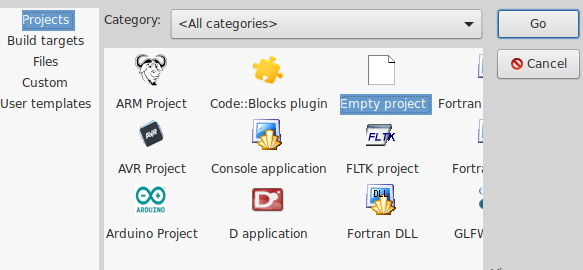
\includegraphics[width=0.4\linewidth]{images/c_cb_1}
			\caption{membuat project kosong}
		\end{figure}
		\item Isi nama project.
		\begin{figure}[H]
			\centering
			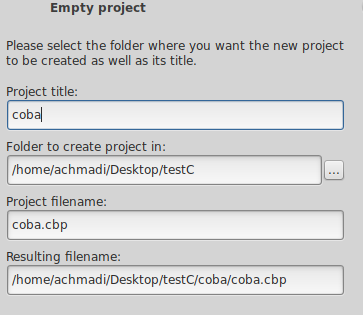
\includegraphics[width=0.4\linewidth]{images/c_cb_2}
			\caption{nama dan tempat project}
		\end{figure}
		\item Pilih compiler \textbf{GNU GCC} dan isi build target \textbf{all} seperti dibawah
		\begin{figure}[H]
			\centering
			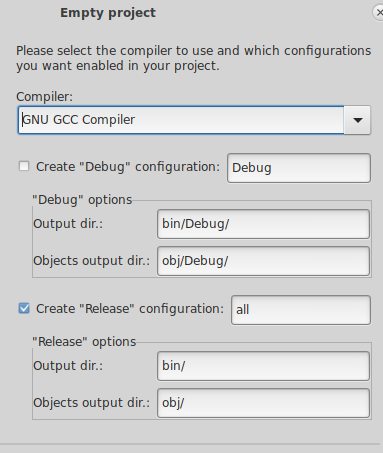
\includegraphics[width=0.4\linewidth]{images/c_cb_3}
			\caption{pilih compiler}
		\end{figure}
		\item Buat File baru
		\begin{figure}[H]
			\centering
			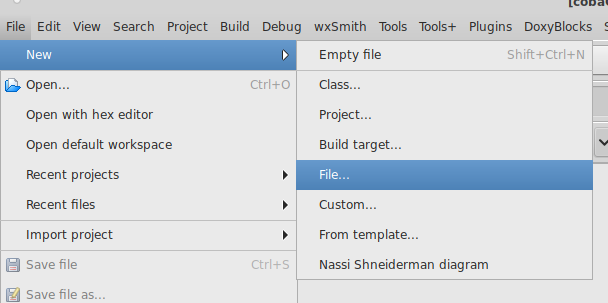
\includegraphics[width=0.4\linewidth]{images/c_cb_4}
			\caption{buat file baru}
		\end{figure}
		\item Pilih file C/C++ Sources
		\begin{figure}[H]
			\centering
			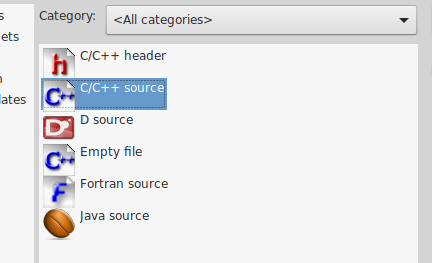
\includegraphics[width=0.4\linewidth]{images/c_cb_5}
			\caption{C/C++ source}
		\end{figure}
		\item Pilih tipe C
		\begin{figure}[H]
			\centering
			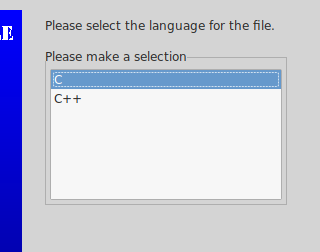
\includegraphics[width=0.4\linewidth]{images/c_cb_6}
			\caption{C source}
		\end{figure}
		\item isi alamat folder project tadi diakhiri dengan \textbf{main.c}.
		Jangan lupa centang \textbf{all} untuk menambahkan file ke 
		\begin{figure}[H]
			\centering
			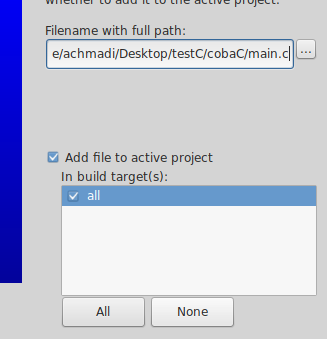
\includegraphics[width=0.4\linewidth]{images/c_cb_7}
			\caption{nama dan alamat file}
		\end{figure}
		\item hasil akhir \textbf{main.c}.
		\begin{figure}[H]
			\centering
			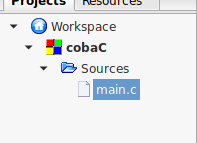
\includegraphics[width=0.4\linewidth]{images/c_cb_8}
			\caption{file main.c}
		\end{figure}
	
		\item masukkan kode berikut.
		Tips: Manfaatkan Code Compeletion.
		\begin{minted}[frame=lines,fontsize=\footnotesize]{c}
#include <stdio.h>

int main() {
	printf("Hello, World! \n");
	return 0;
}
		\end{minted}
		\item Tekan menu Build->Build and Run.
		\begin{figure}[H]
			\centering
			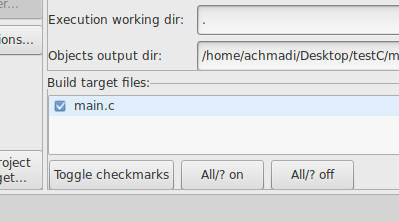
\includegraphics[width=0.4\linewidth]{images/c_cb_9}
			\caption{Build and Run}
		\end{figure}
			
	\end{enumerate}

	\subsubsection{Tipe Data}
	Tipe data dalam bahasa C diukur dengan satuan \textbf{bit}.
	Nilai 1 bit adalah nilai terkecil dalam memory yang bisa diisi antara 1 atau 0 (salah satu).
	Berikut satuan tipe data yang sering dipakai:
	\begin{itemize}
		\item Bit. Satuan terkecil yang hanya berisi 1 atau 0
		\item Nibble. Senilai dengan 4bit.
		\item Byte. Senilai dengan 8bit.
	\end{itemize}

	Selanjutnya dalam alokasi variable dalam memory, dikenal istilah tipe data.
	Tipe data adalah deklarasi jenis variable berdasarkan ukurannya.
	Setiap tipe data memiliki ukuran maximal yang jika nilai nya melewatinya akan terjadi \textit{overflow} (kembali ke 0).
	Berikut tipe data yang umum:
	\begin{table}[H]
		\begin{tabular}{|l|l|l|l|l}
			\cline{1-4}
			\textbf{name}      & \textbf{type}          & \textbf{bit-size} & \textbf{range}         &  \\ \cline{1-4}
			boolean   & bool          & 1  & 0$\sim$1             &  \\ \cline{1-4}
			character & unsigned char & 8  & 0$\sim$255           &  \\ \cline{1-4}
			character & char          & 8  & -127$\sim$128        &  \\ \cline{1-4}
			integer   & unsigned int  & 16 & 0$\sim$65.535        &  \\ \cline{1-4}
			integer   & int  		  & 16 & -32,768$\sim$32,767  &  \\ \cline{1-4}
			long	  & unsigned long & 32 & 0$\sim$4,294,967,295 &  \\ \cline{1-4}
			long	  & long 		  & 32 & $\pm$2,147,483,647	  &  \\ \cline{1-4}
			float	  & float 		  & 32 & $\pm$2,147,483,647	  &  \\ \cline{1-4}
			double	  & double 		  & 64 & $\pm$9,223,372,036,854,775,807	&  \\ \cline{1-4}
		\end{tabular}
	\end{table}
	Untuk tipe double dan float, mampu menyimpan bilangan \textit{floating-point} (decimal).
	Akan tetapi standar floating-point setiap chip arsitektur berbeda-beda sehingga perlu diperhatikan.
	
	Tujuan setelah mengenal tipe data adalah untuk mendeklarasikan tipe variabel sesuai kebutuhan.
	Dalam bahasa C/C++, variable wajib dideklarasikan terlebih dahulu agar sistem dapat memesan ukuran memori secara pas.
	Pola deklarasi variable:
	\begin{minted}[frame=lines,fontsize=\footnotesize]{c}
<rentang> <tipedata> variabel;
	\end{minted}
	Penjelasan:
	\begin{itemize}
		\item <rentang> adalah tipe rentang yang dipakai.
		Pilihannya adalah \textbf{unsigned} yaitu dari 0 hingga maximal.
		Dan \textbf{signed} atau \textbf{kosong} saja untuk minus setengah maximal hingga plus setengah maximal.
		\item <tipedata> adalah tipe data sesuai rentang.
		\item variabel adalah nama variable dengan aturan:
		\begin{itemize}
			\item tidak diawali angka, tapi boleh underscore (\_).
			\item tidak boleh ada spasi,koma,titik, tapi boleh underscore (\_).
			\item tidak konflik nama dengan yang lain di lingkungan pemrograman.
		\end{itemize}
	\end{itemize}

	Sebagai contoh:
	\begin{minted}[frame=lines,fontsize=\footnotesize]{c}
unsigned int foo;
foo = 5;
int foomin;
foomin = -5;
	\end{minted}
	
	
	
\end{document}